\section{Evaluation} \label{section:evaluation}


\begin{figure}[t]
\centering
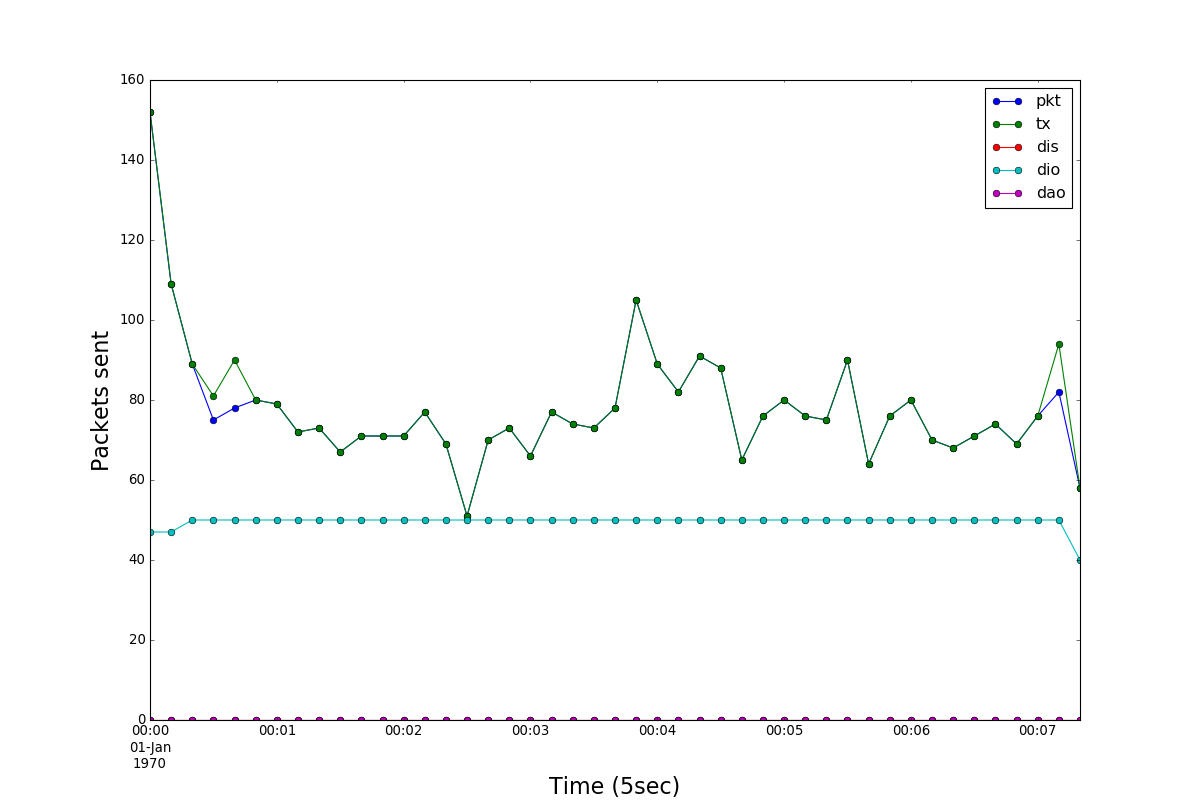
\includegraphics[width=\linewidth]{figs/rpl_single_hop.png}
\caption{Sum of packet types sent over time over all nodes in a RPL topology of a single broadcast domain.}
\label{fig:rpl_single_hop}
\end{figure}

\begin{figure}[t]
\centering
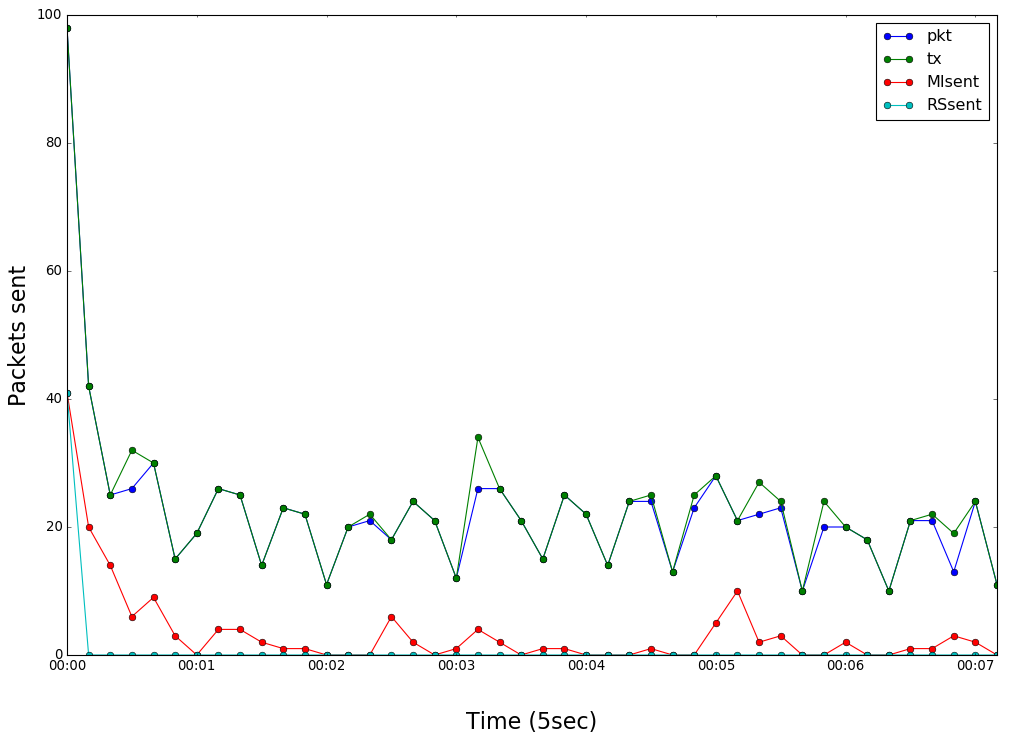
\includegraphics[width=\linewidth]{figs/3hop_single_hop.png}
\caption{Sum of packet types sent over time over all nodes in a 3hop topology of a single broadcast domain.}
\label{fig:3hop_single_hop}
\end{figure}

\begin{figure}[t]
\centering
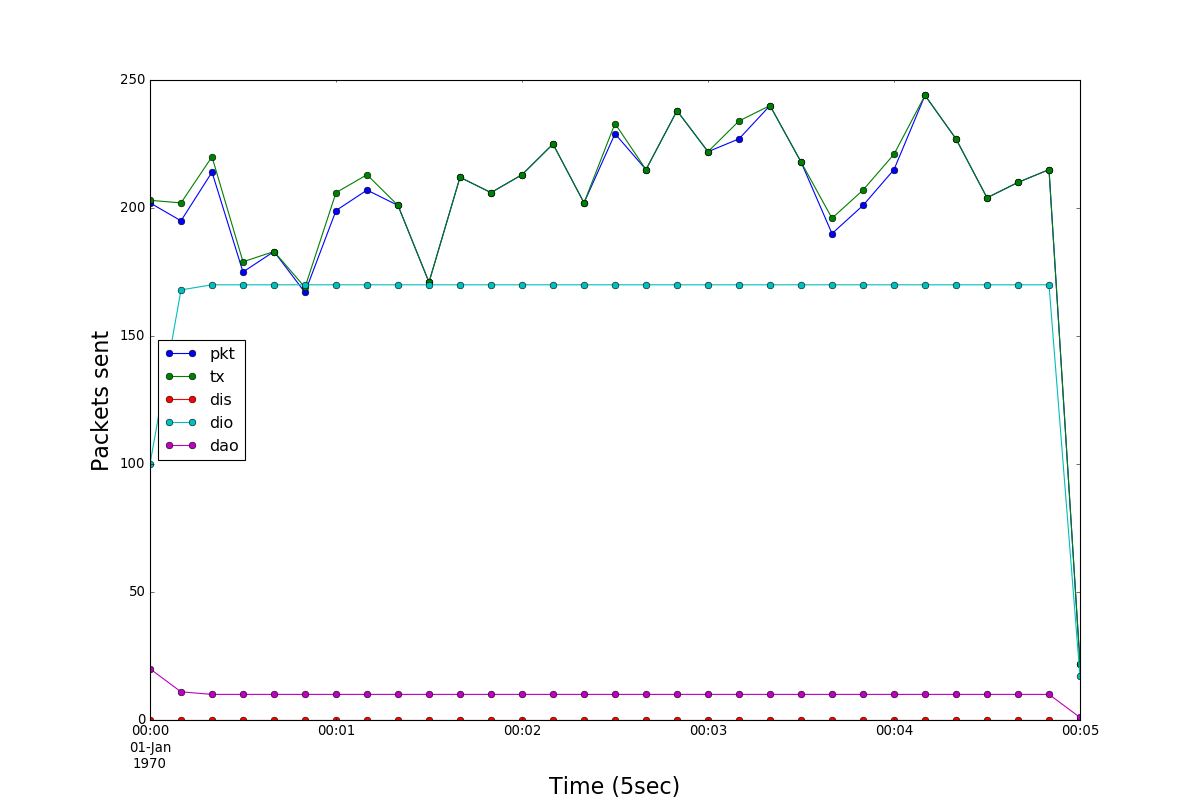
\includegraphics[width=\linewidth]{figs/rpl_multi_hop.png}
\caption{Sum of packet types sent over time over all nodes in a multi-hop RPL topology}
\label{fig:rpl_multi_hop}
\end{figure}

\begin{figure}[t]
\centering
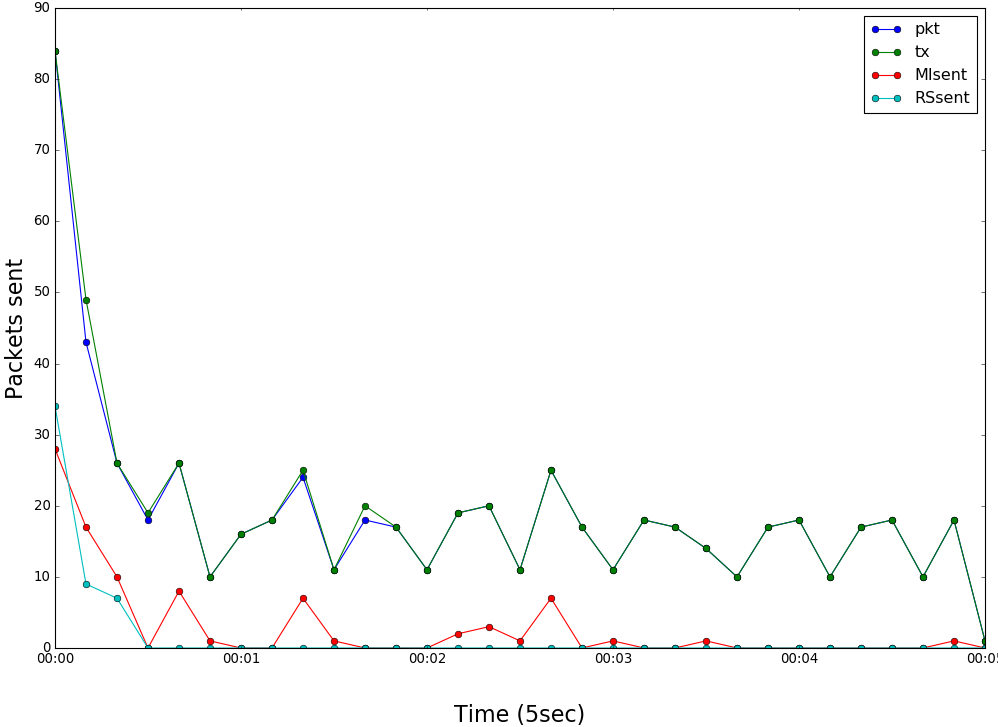
\includegraphics[width=\linewidth]{figs/3hop_multi_hop.png}
\caption{Sum of packet types sent over time over all nodes in a multi-hop 3hop topology}
\label{fig:3hop_multi_hop}
\end{figure}

Lastly, we present an initial evaluation of the 3hop routing protocol in comparison to the RPL routing protocol standard.
Though this is by no means a comprehensive evaluation, we provide evidence that that the 3hop protocol generates less control traffic and results in a better packet reception ratio for realistic application traffic rates.

\subsection{Methodology}

\begin{table}[t]
\centering
\caption{Summary of the results from the four network scenarios using both RPL and 3hop in a single broadcast domain deployment and a multihop deployment}
\label{table:results}
\begin{tabular}{|l|l|l|l|}
\hline
\textbf{Experiment} & \textbf{Reported/Total} & \textbf{PRR min/max} & \textbf{PRR mean/std} \\
\hline
\hline
RPL Single Hop & 10 / 10 & 36\% / 100\% & 82\% / 21\% \\
3hop Single Hop & 10 / 10 & 97\% / 100\% & 98\% / 1\% \\
RPL Multi Hop & 8 / 10 & 48\% / 51\% & 50\% / 1\% \\
3hop Multi Hop & 10 / 10 & 86\% / 100\% & 95\% / 4\% \\
\hline
\end{tabular}
\end{table}


All experiments here were run in an 11 node configuration, with one of the nodes performing as a dedicated border router and root node.
The other 10 nodes generate application traffic at the rate of a single (non-fragmented) packet sent to a server outside the network every 30 seconds.
This packet contains a monotonically increasing counter which is logged at the server and allows us to calculate the packet reception ratio (PRR).
During the experiment, each node also logs the set of transmitted packets, retransmissions and counts of routing protocol control traffic over time; during the reporting phase each node replay this log and relays the data to the coordinating server.
The network measurement platform takes one sample every 5 seconds.
These logs generate the graphs in Figures~\ref{fig:rpl_single_hop}, \ref{fig:3hop_single_hop}, \ref{fig:rpl_multi_hop} and \ref{fig:3hop_multi_hop}.
To accentuate the control traffic patterns, these graphs are smoothed with by taking the sum of packets per traffic type in 10-second buckets. Raw data is available at \url{https://github.com/gtfierro/cs268-project/tree/master/capture}.

For each routing protocol --- RPL and 3hop --- we execute this scenario for two topologies:
\begin{itemize}
\item Single-hop: all nodes were placed in a 1 sq foot area next to the border router.
In this scenario, \emph{there is no need for a routing protocol}, so the vital metric is how well the routing protocol can ``get out of the way'' of the application traffic.
\item Multi-hop: all nodes were distributed over an approx $6\times 14$ meter lab space with metal desks, cabinets and other obstructions assisting the formation of a multi-hop topology.
In this scenario, the primary metric is the packet delivery ratio (which is assumed to be high in the single-hop case).
\end{itemize}

The results of the experiements are summarized in Table~\ref{table:results}.
For the RPL experiments, we configured the nodes to use the OF0 objective function to make it more comparable to the hop-count metric of 3hop.
All RPL nodes additionally use the ``storing'' mode of operation, meaning they maintain downwards as well as upwards.

\subsection{Single-Hop}

While both protocols achieve similar packet reception ratios, the RPL topology generates roughly twice as many packets because of the constant overhead of DIO advertisement messages.
In contrast, the 3hop protocol generates its equivalent of DIO --- the Router Advertisement messages with the Mesh Info option --- on a Trickle timer, thus reducing the portion of traffic related to maintenance of the topology.
We do not observe any DIS messages in the RPL deployment, perhaps due to the constant stream of DIOs suppressing that message.
In the 3hop scenario, each node only sends a single Router Solicitation message before joining the mesh.

\subsection{Multi-Hop}

In the multi-hop case, RPL behaves according to our expectations: because there are multiple hops in the network, the packet transmission counts are higher.
We also see DAO traffic being sent by the motes that are more than one hop away from the root node.
Surprisingly, the amount of DIO traffic, while still constant, is higher than in the single hop scenario, suggesting that the TinyOS RPL implementation does not have a mechanism for reducing control traffic.
For both the DAO and DIO traffic, the RPL specification is vague enough that although we can clearly see the incurred overhead and its detrimental effects on PRR (a dismal 50\% average), this implementation is still ``standards compliant''.

Conversely, the 3hop protocol performs similar to the single-hop scenario: control traffic quiesces gracefully as the nodes share state, and PRR is high and consistent across the nodes.
